%!TEX root=../documentation-bachlorthesis-speicherarchitektur-lstucker.tex
\cleardoublepage
\chapter{Evaluation}

\section{Soll-Kriterien festlegen}
Die gewählten Kriterien für die Evaluation wurden Zusammen mit dem Auftraggeber im Meeting festgelegt. In einen weiteren schritt, sind die einzelnen Kriterien nach ihren Logischen Zugehörigkeit hierarchisch geordnet und verfeinert (\refabb{abb:AHPKriterienbaum}). Die Überarbeitete Kriterien Auswahl wurde bei einen weiteren Meeting mit dem Auftraggeber besprochen und fixiert. 

Die Kriterien sind für die spätere Verweise die Verweise Hierarchisch-Nummeriert.

\begin{center}
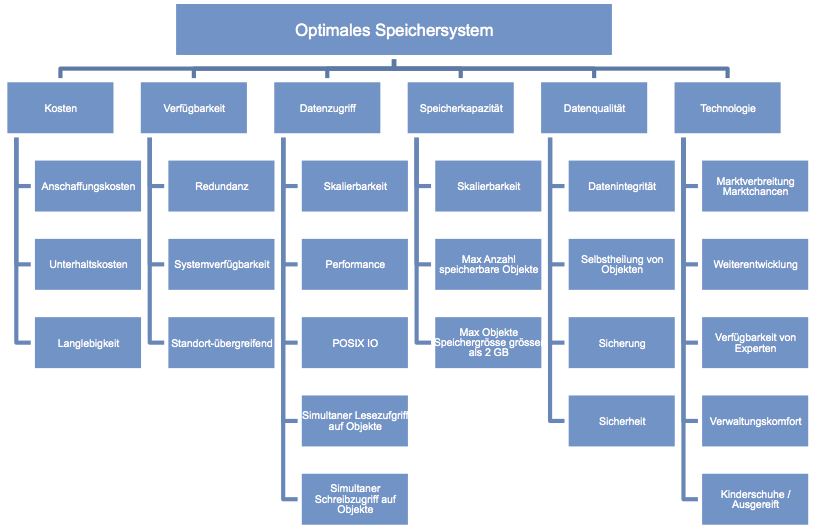
\includegraphics[width=\linewidth, keepaspectratio = true]{media/ahp_kirterienbaum.png}
\mycaption{figure}{\label{abb:AHPKriterienbaum} Optimales Speichersystem Kriterien}
\end{center}

\subsection{Haupt Soll-Kriterien festlegen}
Die Haupt-Kriterien sind auf der obersten Hierarchie Ebene und werden durch Ihre unter Kriterien definiert.
\setcounter{paragraph}{0}
\renewcommand\theparagraph{Soll-\arabic{paragraph}}
\paragraph{Kosten}\label{Soll-1}
Die Kosten sollen das Kostendach von ??? nicht überschreiten. 

\paragraph{Verfügbarkeit}\label{Soll-2}
Die Verfügbarkeit der Daten soll in Bezug auf die Szenerien die Verfügbarkeit erfüllen können. 

\paragraph{Datenzugriffe}\label{Soll-3}
Der Datenzugriff soll Skalieren können, dass heisst es soll möglich sein von mehren Webserver auf den Datenspeicher zugreifen zu können. Der Datenzugriff soll über POSIX IO oder über eine Dokumentiertes API erfolgen können.

\paragraph{Speicherkapazität}\label{Soll-4}
Die Speicherkapazität soll die Speicheranforderungen der Szenerien erfüllen können. Zudem sollen die Speicherung von Grossen Dateien bis mindestens 2 Gigabyte möglich sein.

\paragraph{Datenschutz}\label{Soll-5}
Der Datenschutz der Daten soll gewährleistet werden, dabei gilt das Haupt Augenmerk auf die Unveränderbarkeit der Gespeicherten Daten. Wichtig für den Auftraggeber ist ebenfalls das die Datengesichert werden können.

\paragraph{Technologie}\label{Soll-6}
asdf

\subsection{Unter Soll-Kriterien festlegen}
Die unter Kriterien mit den gleichen Nummer-Ebene gehören zusammen zur gleichen oben-Kriterien und werden später bei der Gewichtung der Kriterien nur untereinander direkt Verglichen.

\setcounter{paragraph}{0}
\renewcommand\theparagraph{Soll-1-\arabic{paragraph}}

\paragraph{Anschaffungskosten}\label{Soll-1-1}

\paragraph{Unterhaltskosten}\label{Soll-1-2}

\paragraph{Nachhaltigkeit}\label{Soll-1-3}

\setcounter{paragraph}{0}
\renewcommand\theparagraph{Soll-2-\arabic{paragraph}}

\paragraph{Redundanz}\label{Soll-2-1}
Die redundante Haltung der aktiven Daten, dass heisst der Daten die Aktive zugegriffen und manipuliert werden können, Dient zur Erhöhung der Verfügbarkeit der Daten bei einen Komponenten Ausfall. Die doppelt Haltung der Daten zur Sicherungszwecken, wie Archivierung wird nicht als redundant erachtet, da diese nicht direkt zu einer Erhöhung der System Verfügbarkeit ohne Menschliche Unterstützung führt. Die Speicherlösung sollte mindestens die Daten doppelt, wenn möglich dreifach Redundanz halten. 


\paragraph{Systemverfügbarkeit}\label{Soll-2-2}
Die Systemverfügbarkeit, wird durch Software oder Hardware Redundanz erreicht. Das System soll möglichst Redundant ausgelegt sein um eine Verfügbarkeit nach AEC-3 Standard zu erreichen.

\paragraph{Standort-übergreifend}\label{Soll-2-3}
Die aktive Daten sollen nach Möglichkeit an mindesten zwei Standorte verfügbar sein, um den Dienst bei einen Ausfall eines Rechenzentrums aufrecht zu erhalten können.

\setcounter{paragraph}{0}
\renewcommand\theparagraph{Soll-3-\arabic{paragraph}}

\paragraph{Skalierbarkeit}\label{Soll-3-1}
Die Speicherlösung sollte bei bedarf Ihren Speicher an bis zu 30 Serversysteme zur Verfügung stellen können.

\paragraph{Performance}\label{Soll-3-2}
Die Speicherlösung soll eine IO Performance von mindesten 27.31 MBit pro Sekunde haben.

\paragraph{POSIX IO}\label{Soll-3-3}
Die POSIX IO (inoffizielle Bezeichnung) ist eine Teil des POSIX Standards welche die IO Schnittstelle für POSIX Kompatible Applikationen definiert. Der Standard definiert unteranderem die Funktionen read(), write(), open(), close() inklisive deren Fehler Behandlung. Die Speicherlösung soll, für eine einfache Implementierung, nach Möglichkeit diesen Standard unterstützen. 

\paragraph{Simultaner Lesezugriff auf Objekte}\label{Soll-3-4}
Das gleichzeitige Lesen auf das selbe Objekte von zwei oder mehrere Serversysteme soll möglich sein.

\paragraph{Simulataner Schreibzugriff auf Objekte}\label{Soll-3-5}
Das gleichzeitige schreiben auf das selbe Objekte von zwei oder mehrere Serversysteme soll optional möglich sein.

\setcounter{paragraph}{0}
\renewcommand\theparagraph{Soll-4-\arabic{paragraph}}

\paragraph{Skalierbarkeit}\label{Soll-4-1}

\paragraph{Max Anzahl speicherbare Objekte}\label{Soll-4-2}
Das Speicherlösung soll die Anzahl Speicherbaren Objekten der Soll-Zenarien unterstützen. 

\paragraph{Max Objekte Speichergrösse grösser als 2 GB}\label{Soll-4-3}
Das Speichersystem muss die Speicherung von Objekten mit einer Speichergrösse von mindestenz 2 GigaByte unterstützen.

\setcounter{paragraph}{0}
\renewcommand\theparagraph{Soll-5-\arabic{paragraph}}

\paragraph{Datenintegrität}\label{Soll-5-1}
Die Datenintegrität der gespeicherten Daten soll gewährleistet sein.

\paragraph{Selbstheilung von Objekten}\label{Soll-5-2}
Die Selbstheilung von nicht mehr integer Daten soll nach Möglichkeit unterstützt werden. Diese Funktion ist bei der Verwaltung von grossen Datenmengen eine unterstützende Funktion.

\paragraph{Datensicherung}\label{Soll-5-3}
Die gespeicherten Daten soll mit einen Sicherungsverfahren gesichert werden können. Wenn die aktiven Daten nicht an zwei Standorten zur Verfügung gestellt werden können, wie in (\refsoll{Soll-2-3}) definiert, ist es zwingen erforderlich das die Sicherung an einen zweiten Standort erfolgen kann.

\paragraph{Datensicherheit}\label{Soll-5-4}
Die Datenberechtigung wird in der Applikation Implementiert, die Speicherlösung soll nach Möglichkeit Sicherstellen, das die Daten nicht von dritten Zugegriffen werden kann.

\setcounter{paragraph}{0}
\renewcommand\theparagraph{Soll-6-\arabic{paragraph}}

\paragraph{Marktverbreitung / Marktchancen}\label{Soll-6-1}
Die Speicherlösung soll im Markt verbreitet sein oder Tendenzen aufweisen die auf eine Verbreiterung im Markt in den nächsten fünf Jahren schliessen lässt.

\paragraph{Weiterentwicklung}\label{Soll-6-2}
Die Speicher Technologien welche aktive Weiterentwickelt werden soll hoher bewertet werden als Speicherlösung Technologie welche nicht mehr weiter gepflegt werden.

\paragraph{Verfügbarkeit von Experten}\label{Soll-6-3}
Die Verfügbarkeit von Experten Speicherlösungstechnologie soll gegeben sein. Dabei ist das Experten Wissen auch nach Verfügbarkeit nach Lokalität zu bewerten. Die Verfügbarkeit von Experten im Raum Schweiz ist höher zu werten als im Raum Europa.

\paragraph{Verwaltungskomfort}\label{Soll-6-4}
Die Speichertechnologie soll die geforderte Datenmenge mit möglichst geringen Aufwand komfortable verwalten lassen.

\paragraph{Kinderschuhe / Ausgereift}\label{Soll-6-5}
Die Speicher Technologie soll Ausgereift und Stabil laufen. Eine Implementierung von Beta Technologie ist nicht erwünscht.
Die Technologie soll Ausgereift sein, bzw. keine erst Implementierung.

\section{KO-Kriterien}
Die KO-Kriterien sind muss Kriterien die von einen Speichersystem erfüllt werden müssen. Speichersysteme welche die KO-Kriterien nicht erfüllen werden bei der AHP-Evaluation ausgeschlossen. Die KO-Kriterien wurde zusammen mit dem Auftraggeber besprochen und vereinbart.

\setcounter{paragraph}{0}
\renewcommand\theparagraph{KO-\arabic{paragraph}}

\paragraph{Dateigrösse bis 2 Gigibyte}
Die Speicherung von Dateien die eine Speichergrösse von 2 Gigibyte muss unterstützt werden.

\paragraph{Speicherkapazität Szenarien}
Die geforderten Speicherkapazitäten der Szenerien inklusive die benötigte Kapazität für die Redundanz muss von der Speicherlösung unterstützt werden.

\paragraph{System Redundanz}
Das Speichersystem soll auf mehren Systemen betrieben werden können.

\section{Auswahl der Alternativen / Vertreter}
Mit dem Auftraggeber wurde definiert, dass aus den Speicherlösung, SAN, NAS, Distributed Filesystem Cluster, Online Speicher und   Dedizierter Server Webserver einen Vertreter für die Evaluation ausgewählt werden soll. Die Lösungen wurden nach Marktverbreitung, Technologie Leader ausgewählt.

Die Alternativen/ Vertreter sind für die spätere Verweise die Verweise Nummeriert.

\setcounter{paragraph}{0}
\renewcommand\theparagraph{Al-\arabic{paragraph}}

\paragraph{NetApp}\label{Al-1}
Als Vertreter für die NAS Speicherlösung wurde Netapp xxx ausgewählt. Die Firma Netapp gehört mit ihren NAS Speicherlösung zu den Markführer (siehe \refsec{MartkEtabliert}) und gelten als 

\paragraph{NetApp}\label{Al-2}

\paragraph{Hadoop}\label{Al-3}
Als Vertreter für Distributed Filesystem wurde das 

\paragraph{Open-Stack Swift}



\paragraph{Amazone S3}
Als Vertreter für Online Speicherlösung (Cloud Storage) gewählt. Amazon gilt als Führender Anbieter in Bereich Cloud Lösungen (siehe \\refsec{MartkEtabliert} und betreibt Rechenzentren den Vereinigten Staaten, Europa und Asien. 

\paragraph{Hetzner}\label{Al-3}
Dedizierte Webserver zählen im engeren Sinn nicht als reine Speicherlösungen, der Deutsche Hosting Anbieter Hetzner bietet jedoch Dedizierte Webserver mit einer Speicherkapazität welche die Anforderung an die Kapazität des Szenario 1 (siehe \refsec{Szenario1}) erfüllen. Hetzner als Dedizierter Webserver Anbieter wurde ausgewählt, weil die bestehende Lösungen ebenfalls mit Hetzer Webserver realisiert ist. Root Server XS 29


\subsection{Gewichtung der Soll-Kriterien mit AHP}

% Vergleich mit Kosten
\paragraph*{\refsoll{Soll-1} verglichen mit \refsoll{Soll-2} (\ref{Soll-1}/\ref{Soll-2})} 
Mit steigenden Anforderungen an die Verfügbarkeit steigen auch die Kosten. Der Betrieb einer Infrastruktur eines Service Anbieters muss Kostendecken sein. Einen Ausfall des System während definierten Zeiten in welches das System Online sein muss, hat ebenfalls Auswirkungen auf das Unternehmen. So kann es zum Image Verlust, zu Kunden Abgänge führen, oder die Zahlung von Entschädigung erfordern. Einen Datenverlust kann trotzt Sicherungskopie bei Grossen Datenmengen zeitintensive und kostspielig werden. Aus diesen Gründen ist eine gute Balance zwischen Kosten und Verfügbarkeit zu finden. Die Kosten sind deshalb im Vergleich zur Verfügbarkeit etwas grösser zu Gewichten.

\textbf{Gewichtung: 3}

\paragraph*{\refsoll{Soll-1} verglichen mit \refsoll{Soll-3} (\ref{Soll-1}/\ref{Soll-3})}

\paragraph*{\refsoll{Soll-1} verglichen mit \refsoll{Soll-4}}

\paragraph*{\refsoll{Soll-1} verglichen mit \refsoll{Soll-5}}
Die Kosten werden als 
\paragraph*{\refsoll{Soll-1} verglichen mit \refsoll{Soll-6}}

% Vergleich mit Verfügbarkeit
\paragraph*{\refsoll{Soll-2} verglichen mit \refsoll{Soll-3}}
Aus Sicht des Anwenders ist die Verfügbarkeit der Daten höher zu Gewichten als möglichst schnellen Zugriff oder die Art und weise wie zugegriffen wird. Allerdings kann eine langes Zeitüberschreitung beim ausliefern der Daten für den Anwender ebenfalls als nicht Verfügbarkeit empfunden werden. Die Verfügbarkeit ist zwischen etwas Grösser bis erheblich Grösser zu Gewichten als der Datenzugriff.

\textbf{Gewichtung: 4}

\paragraph*{\refsoll{Soll-2} verglichen mit \refsoll{Soll-4}}
Zum Geschäftsmodell des Auftraggeber gehört unter anderem die Bereitstellung von Speicherkapazität für die Speicherung der Bilddaten seiner Kunden. Sind die Speicherkapazitäten ausgeschöpft ist es dem Auftraggeber nicht mehr möglich in diesen Geschäftsbereich weiter zu Wachsen. Aus diesen Grund ist die Verfügbarkeit etwas geringere zu Gewichten als die Speicherkapazität.

\textbf{Gewichtung: 1/3}


\paragraph*{\refsoll{Soll-2} verglichen mit \refsoll{Soll-5}}

\paragraph*{\refsoll{Soll-2} verglichen mit \refsoll{Soll-6}}


% Vergleich mit Datenzugriffe
\paragraph*{\refsoll{Soll-3} verglichen mit \refsoll{Soll-4}}

\paragraph*{\refsoll{Soll-3} verglichen mit \refsoll{Soll-5}}

\paragraph*{\refsoll{Soll-3} verglichen mit \refsoll{Soll-6}}

% Vergleich mit Speicherkapazität
\paragraph*{\refsoll{Soll-4} verglichen mit \refsoll{Soll-5}}

\paragraph*{\refsoll{Soll-4} verglichen mit \refsoll{Soll-6}}

% Vergleich mit Datenschutz
\paragraph*{\refsoll{Soll-5} verglichen mit \refsoll{Soll-6}}




\begin{table}[htbp]
\caption{AHP Gewichtung Top Kriterien}
\begin{tabular}{|l|c|c|c|c|c|r|r|}
\hline
\multicolumn{ 1}{|c|}{} & \multicolumn{ 5}{c|}{Evalutations Matrix} & \multicolumn{1}{l|}{} & \multicolumn{1}{l|}{Gewicht} \\ \cline{ 2- 8}
\multicolumn{ 1}{|c|}{} & K & V & P & S & D & \multicolumn{1}{c|}{r} & \multicolumn{1}{c|}{w} \\ \hline
Kosten (K) & \textbf{1} & 2 & 3 & 1 & 1 & 1.131 & 0.226 \\ \hline
Verfügbarkeit (V) &  1/2 & \textbf{1} & 5 &  1/3 &  1/8 & 0.569 & 0.114 \\ \hline
Performance (P) &  1/3 &  1/5 & \textbf{1} &  1/4 &  1/7 & 0.257 & 0.051 \\ \hline
Speicherkapazität (S) & 1 & 3 & 4 & \textbf{1} &  1/2 & 1.071 & 0.214 \\ \hline
Datenqualität (D) & 1 & 8 & 7 & 2 & \textbf{1} & 1.972 & 0.394 \\ \hline  \hline
Ci & \multicolumn{1}{r|}{3.833} & \multicolumn{1}{r|}{14.200} & \multicolumn{1}{r|}{20.000} & \multicolumn{1}{r|}{4.583} & \multicolumn{1}{r|}{2.768} & 5 & 1 \\ \hline 
\end{tabular}
\label{AHPTop}
\end{table}

\paragraph*{\refsoll{Soll-1-1} verglichen mit \refsoll{Soll-1-2} (\ref{Soll-1-1}/\ref{Soll-1-2})}
Die Betriebskosten sind der Hauptkostenfakor in der Lebenszeit eines Informations-Systems. Gemäss Gartner vielen die Weltweiten IT-Kosten im Jahr 2011 zu 20\% für die Computer Hardware und zu 43\% IT-Service an. Zudem Steigen die Kosten zum Beispiel von Disk Array Speicher nach Ablauf der ordentlichen von Hersteller gewährleisteten Wartung, wegen teuren weiterführenden Wartungsverträge stark an.
Aus diesen Grund sind die Anschaffung Kosten im vergleich zur Unterhaltskosten erheblich geringer zu Gewichten.

\textbf{Gewichtung: 1/5}

\paragraph*{\refsoll{Soll-1-1} verglichen mit \refsoll{Soll-1-3} (\ref{Soll-1-1}/\ref{Soll-1-3})}
Fällt die Langlebigkeit eines Systems, weil es technologisch veraltet ist oder weil die Kosten für Wartungsverträge nach Ablauf der ordentlichen Wartung im Vergleich zur neu Anschaffung unrentabel sind, kurz aus. Sind erneut Kosten in der Anschaffung und Migration der Daten notwendig. Aus diesen Grund sind die Anschaffungskosten im Vergleich zur Langlebigkeit etwas geringer zu Gewichten.

\textbf{Gewichtung: 1/3}


\paragraph*{\refsoll{Soll-1-2} verglichen mit \refsoll{Soll-1-3} (\ref{Soll-1-2}/\ref{Soll-1-3})}
Der Hauptkostenfakor in der Lebenzeit eines Information System sind die Betreibskosten, steigen diese Kosten Aufgrund hoher Wartungverträgekosten mit der Lebenspanne des Systems an, kann sich der Betrieb als unrentable herausstellen. Aus diesen Grund sind die Betriebskosten im Vergleich zu Langlebigkeit etwas grösser zu Gewichten.

\textbf{Gewichtung: 3}

\begin{table}[htbp]
\caption{AHP Kosten}
\begin{tabular}{|l|c|c|c|r|r|}
\hline
\multicolumn{ 1}{|c|}{Wirtschaftlichkeit} & \multicolumn{ 3}{c|}{Evalutations Matrix} & \multicolumn{1}{l|}{} & \multicolumn{1}{l|}{Gewicht} \\ \cline{ 2- 6}
\multicolumn{ 1}{|c|}{} & A & U & L & \multicolumn{1}{c|}{r} & \multicolumn{1}{c|}{w} \\ \hline
Anschaffung (A) & \textbf{1} &  1/4 &  1/3 & 0.368 & 0.123 \\ \hline
Unterhaltskosten (U)  & 4 & \textbf{1} & 2 & 1.671 & 0.557 \\ \hline
Langlebigkeit (L) & 3 &  1/2 & \textbf{1} & 0.961 & 0.320 \\ \hline \hline 
Ci & \multicolumn{1}{r|}{8.00} & \multicolumn{1}{r|}{1.750} & \multicolumn{1}{r|}{3.333} & 3 & 1 \\ \hline
\end{tabular}
\label{AHPKosten}
\end{table}


\paragraph*{\refsoll{Soll-2-1} verglichen mit \refsoll{Soll-2-2} (\ref{Soll-2-1}/\ref{Soll-2-2})}
Die Daten eines Informationssystem sind dessen wertvollstes Gut, mit höherer Redundanz der Daten steigt auch die Verfügbarkeit der Daten.
Die Gesamt Verfügbarkeit hängt jedoch auch von der Verfügbarkeit der System Komponenten zusammen. Aus diesen Grund sollten die Daten System übergreifend Redundant sein um eine hohe Verfügbarkeit zu erreichen. Gemäss eigener Erfahrungen, ist die Zahl der Datenträger ausfälle höher als die restlichen Komponenten ausfälle eines Systems. Die Datenredundanz ist deshalb erheblich grösser zu Gewichten als die System Redundanz.

\textbf{Gewichtung: 5}

\paragraph*{\refsoll{Soll-2-1} verglichen mit \refsoll{Soll-2-3} (\ref{Soll-2-1}/\ref{Soll-2-3})}
Die Standortübergreifende Verfügbarkeit der Daten kann nur mit Redundanz der Daten erreicht werden, aus diesen Grund ist die Datenredundanz absolut höher zu Gewichten als die Standortübergreifende Verfügbarkeit.

\textbf{Gewichtung: 9}

\paragraph*{\refsoll{Soll-2-2} verglichen mit \refsoll{Soll-2-3} (\ref{Soll-2-2}/\ref{Soll-2-3})}
Die Standortübergreifende Verfügbarkeit des System kann nur mit höherer Systemverfügbarkeit erreicht werden. Aus diesen Grund ist die Redundanz der sehr viel höher zu Gewichten als die Standortübergreifende Verfügbarkeit.

\textbf{Gewichtung: 7}

\begin{table}[htbp]
\caption{AHP Verfügbarkeit}
\begin{tabular}{|p{7.1cm}|c|c|c|r|r|}
\hline
\multicolumn{ 1}{|c|}{Verfügbarkeit} & \multicolumn{ 3}{c|}{Evalutations Matrix} & \multicolumn{1}{l|}{} & \multicolumn{1}{l|}{Gewicht} \\ \cline{ 2- 6}
\multicolumn{ 1}{|c|}{} & R & SV & St & \multicolumn{1}{c|}{r} & \multicolumn{1}{c|}{w} \\ \hline
Redundanz (R) & \textbf{1    } & 8     & 3     & 1.971 & 0.657 \\ \hline
Systemverfügbarkeit (SV) &  1/8 & \textbf{1} &  1/5 & 0.205 & 0.068 \\ \hline
Standortübergreifend (St) &  1/3 & 5     & \textbf{1} & 0.824 & 0.275 \\ \hline \hline
Ci & \multicolumn{1}{r|}{1.458} & \multicolumn{1}{r|}{14.00} & \multicolumn{1}{r|}{4.200} & 3 & 1 \\ \hline
\end{tabular}
\label{AHPVerfügbarkeit}
\end{table}

\paragraph*{\refsoll{Soll-3-1} verglichen mit \refsoll{Soll-3-2} (\ref{Soll-3-1}/\ref{Soll-3-2})}
Die Skalierung der Datenzugriff, dass heisst der Zugriff von mehren Systemen, ermöglicht es die Web-Applikation höher Redundant zu betreiben und die Verarbeitung der Bilddaten auf mehre Server zu Verteilen. Der maximale Datendurchsatz ist daher weniger bedeutend als dessen kostanz bei der Verteilung der Zugriffe auf mehere Server. Aus diesen Grund. Ein Speicherlösung welche schlechte Performance aufweist, skaliert jedoch in der Regel ebenfalls nicht. Aus diesen Grund ist die Skalierung der Datenzugriffe etwas grosser Gewichten als die Performance 

\textbf{Gewichtung: 3}

\paragraph*{\refsoll{Soll-3-1} verglichen mit \refsoll{Soll-3-3} (\ref{Soll-3-1}/\ref{Soll-3-2})}
Ist eine Zugriff auf die Daten über POSIX IO möglich, fällt allenfalls die Anpassung der Entwickelte Web-Applikation geringer aus als wenn er auf die Daten per API zugreifen muss. Für den Betrieb der Web-Applikation ist die Skalierung des Datenzugriffs sehr viel bis absolut bedeutender als die Methode des Datenzugriffs.

\textbf{Gewichtung: 8}


\paragraph*{\refsoll{Soll-3-1} verglichen mit \refsoll{Soll-3-4} (\ref{Soll-3-1}/\ref{Soll-3-4})}
Der Simultaner Lese Zugriff auf ein Objekt ermöglicht es, dass eine Bilddatei von mehren Server simultan gelesen werden kann und den Website Besuchern dargestellt werden kann. Wird diese nicht unterstützt ist es möglich das dem Webseiten Besucher die Bilddatei nicht dargestellt werden kann, wenn ein anderer Besucher die selbe Bilddatei betrachtet. Aus diesen Grund ist die Skalierung und der Simultane Lese Zugriff auf Objekten gleich bedeutend.

\textbf{Gewichtung: 1}


\paragraph*{\refsoll{Soll-3-1} verglichen mit \refsoll{Soll-3-5} (\ref{Soll-3-1}/\ref{Soll-3-5})}
Der Simultaner Schreibzugriff auf ein Objekt erlaubt es, dass eine Objekt simultan von zwei oder mehreren Systemen modifiziert werden kann. Die Web-Applikation des Auftraggeber führt jedoch keine Änderungen an einer Original Bilddatei durch sondern erstellt modifizierte Kopien. Aus diesen Grund ist Möglichkeit der gleichzeitigen Schreibzugriff auf ein Objekt absolut geringer zu Gewichten als die Skalierung des Datenzugriffs

\textbf{Gewichtung: 9}

\paragraph*{\refsoll{Soll-3-2} verglichen mit \refsoll{Soll-3-3} (\ref{Soll-3-2}/\ref{Soll-3-3})}
Für den Betrieb der Web-Applikation ist die Performance der Datenzugriffe sehr viel bedeutender als die Methode des Datenzugriffs.

\textbf{Gewichtung 7}

\paragraph*{\refsoll{Soll-3-2} verglichen mit \refsoll{Soll-3-4} (\ref{Soll-3-2}/\ref{Soll-3-4})}
Die Performance ist erheblich geringer bedeutend als der simultane Lesezugriff auf Objekte. Grund dafür ist das das gleiche Objekte von mehren Web-Server gelesen werden können um diese den Website Besuchern darstellen können 

\textbf{Gewichtung: 1/5}

\paragraph*{\refsoll{Soll-3-2} verglichen mit \refsoll{Soll-3-5} (\ref{Soll-3-2}/\ref{Soll-3-5})}
Aufgrund das keine Manipulationen an der Original Bilddatei durchgeführt wird, ist die Performance der Datenzugriff erheblich höher zu Gewichten als der Simultane Schreib zugriff auf Objekte 

\textbf{Gewichtung: 5}


\paragraph*{\refsoll{Soll-3-3} verglichen mit \refsoll{Soll-3-4} (\ref{Soll-3-3}/\ref{Soll-3-4})}
Die Zugriff Methode der Web-Applikation kann bei bedarf durch die Entwickler angepasst werden. Für den Betrieb der Web-Applikation ist daher die Zugriffs Methode auf die Bilddaten erheblich geringer bedeutend als der Simultane Lese Zugriff.

\textbf{Gewichtung: 1/5}


\paragraph*{\refsoll{Soll-3-3} verglichen mit \refsoll{Soll-3-5} (\ref{Soll-3-3}/\ref{Soll-3-5})}
 Aufgrund das keine Änderungen an Original Bilddateien durchgeführt werden, ist es für den Auftraggeber bedeutender, dass eine Zugriff über POSIX IO möglich ist.

\textbf{Gewichtung: 3}


\paragraph*{\refsoll{Soll-3-4} verglichen mit \refsoll{Soll-3-5} (\ref{Soll-3-4}/\ref{Soll-3-5})}
Die Webapplikation des Auftraggeber führt keine Änderungen an der Original Bilddatei durch, was den Simultaner Schreibzugriff auf Objekten für den Betrieb der Web-Applikation von geringer Bedeutung ist. Der Simultane Lesezugriff auf Objekten muss für den Betrieb der Web-Applikation möglich sein, damit die Bilddaten mehren Websitzungen dargestellt werden können. Aus diesen Grund ist es absolut grosser von Gewicht das ein Simultaner Lesezugriff möglich ist als der Simultaner Schreibzugriff.

\textbf{Gewichtung: 9}

\begin{table}[htbp]
\caption{AHP Gewichtung Datenzugriff}
\begin{tabular}{|p{4.5cm}|c|c|c|c|c|r|r|}
\hline
\multicolumn{ 1}{|c|}{Datenzugriff} & \multicolumn{ 5}{c|}{Evalutations Matrix} & \multicolumn{1}{l|}{} & \multicolumn{1}{l|}{Gewicht} \\ \cline{ 2- 8}
\multicolumn{ 1}{|c|}{} & Sk & P & PIO  & L & S & \multicolumn{1}{c|}{r} & \multicolumn{1}{c|}{w} \\ \hline
Skalierbarkeit (Sk) & \textbf{1} & 2 & 8 & 4 & 5 & 2.193 & 0.439 \\ \hline
Performance (P) &  1/2 & \textbf{1} & 5 &  1/2 &  1/3 & 0.649 & 0.130 \\ \hline
POSIX IO (PIO) &  1/8 &  1/5 & \textbf{1} &  1/9 &  1/7 & 0.152 & 0.030 \\ \hline
Simultaner Lesezufgriff 
auf Objekte (L) &  1/4 & 2 & 9 & \textbf{1} & 3 & 1.149 & 0.230 \\ \hline
Simultaner Schreibzugriff
 auf Objekte (S) &  1/5 & 3 & 7 &  1/3 & \textbf{1} & 0.857 & 0.171 \\ \hline \hline
Ci & \multicolumn{1}{r|}{2.075} & \multicolumn{1}{r|}{8.200} & \multicolumn{1}{r|}{30.00} & \multicolumn{1}{r|}{5.944} & \multicolumn{1}{r|}{9.476} & 5 & 1 \\ \hline
\end{tabular}
\label{AHPDatenzugriff}
\end{table}

\paragraph*{\refsoll{Soll-4-1} verglichen mit \refsoll{Soll-4-2} (\ref{Soll-4-1}/\ref{Soll-4-2})}
Die Skalierung der Speicherkapazität ist gleich zu Gewichten wie die maximal Anzahl Speicherbare Objekt. Beides sind limitierende Faktoren, die bei erreichen der Grenze die Speicherung von neuen Objekten verunmöglichen. Erreicht man die Grenze der Speicherbaren Objekten,  kann der Vorhandene frei Speicherkapazität nicht für neue Objekte verwendet werden. Umgekehrt kann die Speicherkapazität nicht ausgebaut werden, können die frei Kapazität an Speicherbaren Objekten nicht dazu verwendet werden neue Objekte zu Speichern.

\textbf{Gewichtung: 1}

\paragraph*{\refsoll{Soll-4-1} verglichen mit \refsoll{Soll-4-3} (\ref{Soll-4-1}/\ref{Soll-4-3})}
Die Skalierbarkeit der Speicherkapazität, ist für den Betrieb sehr viel grösser zu Gewichten als die Maximale Speichergrösse für Objekte die grösser als 2 Gigibyte sind.

\textbf{Gewichtung: 7}

\paragraph*{\refsoll{Soll-4-2} verglichen mit \refsoll{Soll-4-3} (\ref{Soll-4-2}/\ref{Soll-4-3})}
Die maximale Anzahl speicherbare Objekte, ist für den Betrieb sehr viel grösser zu Gewichten als die Maximale Speichergrösse für Objekte die grösser als 2 Gigibyte sind.

\textbf{Gewichtung: 7}

\begin{table}[htbp]
\caption{AHP Gewichtung Speicherkapazität}
\begin{tabular}{|p{7.1cm}|c|c|c|r|r|}
\hline
\multicolumn{ 1}{|c|}{Speicherkapazität } & \multicolumn{ 3}{c|}{Evalutations Matrix} & \multicolumn{1}{l|}{} & \multicolumn{1}{l|}{Gewicht} \\ \cline{ 2- 6}
\multicolumn{ 1}{|c|}{} & S & A & G & \multicolumn{1}{c|}{r} & \multicolumn{1}{c|}{w} \\ \hline
Skalierbarkeit (S) & \textbf{1} & 1 & 9 & 1.498 & 0.499 \\ \hline
Max Anzahl speicherbare Objekte (A) & 1 & \textbf{1} & 6 & 1.310 & 0.437 \\ \hline
Max Objekt Speichergrösse grösser 2GB (G) &  1/9 &  1/6 & \textbf{1} & 0.192 & 0.064 \\ \hline \hline
Ci & \multicolumn{1}{r|}{2.111} & \multicolumn{1}{r|}{2.167} & \multicolumn{1}{r|}{16.00} & 3 & 1 \\ \hline
\end{tabular}
\label{AHPSpeicherkapazität}
\end{table}

\paragraph*{\refsoll{Soll-5-1} verglichen mit \refsoll{Soll-5-2} (\ref{Soll-5-1}/\ref{Soll-5-2})}
Damit das Speichersystem korrupte Objekte selbständig heilen kann, ist es erforderlich das die Objekte Redundant gespeichert sind und die Integrität der Gespeicherten Objekte geprüft werden kann. Die Integrität der Objekte wird dabei mit einen zuvor erstellten und gespeicherten Hash Prüfsumme verglichen. Aus diesen Grund ist die Datenintegrität erheblich höher zu Gewichten als die Selbstheilung von Objekten.

\textbf{Gewichtung: 5}

\paragraph*{\refsoll{Soll-5-1} verglichen mit \refsoll{Soll-5-3} (\ref{Soll-5-1}/\ref{Soll-5-3})}
Verliert man alle \gls{Primären-Daten} durch einen Hard-, Software Fehler oder durch einwirken von dritten, ist es unerlässlich das eine Sicherungskopie bereit steht um nicht den Total Datenverlust zu erleiden.
Eine weiter Gefahr von Datenverlust besteht, wenn die Datenintegrität nicht sichergestellt ist. Ist ein Objekt nicht mehr integer bzw. korrupt und wird diese vor der Sicherung nicht festgestellt, besteht die Gefahr eines Datenverlustes.
Der Verlust aller Daten ist jedoch schwerwiegender als der Verlust einzelner Daten.
Aus diesen Grund ist die Datenintegrität geringer zu Gewichten als die Datensicherung.

\textbf{Gewichtung: 1/3}

\paragraph*{\refsoll{Soll-5-1} verglichen mit \refsoll{Soll-5-4} (\ref{Soll-5-1}/\ref{Soll-5-4})}
Primär muss bei einer Webapplikation die Sicherheit der Daten innerhalb der Webapplikation sicher gestellt werden. Aus diesen Grund ist die Datenintegrität sehr viel grösser zu Gewichten als Sicherheit.

\textbf{Gewichtung: 7}

\paragraph*{\refsoll{Soll-5-2} verglichen mit \refsoll{Soll-5-3} (\ref{Soll-5-2}/\ref{Soll-5-3})}
Die Selbstheilung von Daten stellt sicher das alle Redundanten gespeicherten \gls{Primären-Daten} integer sind. Durch die Selbstheilung verringert sich das Risiko der eines Datenverlust zu erleiden. 
Der Verlust aller Daten ist jedoch schwerwiegender als der Verlust einzelner Daten.
Aus diesen Grund ist die Selbstheilung der Daten erheblich geringer zu Gewichten als die Datensicherung.

\textbf{Gewichtung: 1/5}

\paragraph*{\refsoll{Soll-5-2} verglichen mit \refsoll{Soll-5-4} (\ref{Soll-5-2}/\ref{Soll-5-4})}
Primär muss bei einer Webapplikation die Sicherheit der Daten innerhalb der Webapplikation sicher gestellt werden. Aus diesen Grund ist die Selbsheilung der Daten erheblich grosser zu Gewichten als Sicherheit.

\textbf{Gewichtung: 5}

\paragraph*{\refsoll{Soll-5-3} verglichen mit \refsoll{Soll-5-4} (\ref{Soll-5-3}/\ref{Soll-5-4})}
Die Datensicherheit ist Primär auf der Web-Applikation Schicht zu gewährleisten und zu realisieren. Erfährt man einen Datenverlust durch einwirken von dritten, ist sicherzustellen das eine Sicherungskopie der Daten existiert. Aus diesen Grund ist die Sicherung der Daten absolut höher zu Gewichten als die Sicherheit.  

\textbf{Gewichtung: 5}

\begin{table}[htbp]
\caption{AHP Gewichtung Datenschutz}
\begin{tabular}{|l|c|c|c|c|r|r|}
\hline
\multicolumn{ 1}{|c|}{Datenqualität} & \multicolumn{ 4}{c|}{Evalutations Matrix} & \multicolumn{1}{l|}{} & \multicolumn{1}{l|}{Gewicht} \\ \cline{ 2- 7}
\multicolumn{ 1}{|c|}{} & I & H & B & S & \multicolumn{1}{c|}{r} & \multicolumn{1}{c|}{w} \\ \hline
Datenintegrität (I) & \textbf{1} & 9 & 3 & 7 & 2.316 & 0.579 \\ \hline
Selbstheilung von Objekten (H) &  1/9 & \textbf{1} &  1/6 &  1/3 & 0.186 & 0.046 \\ \hline
Sicherung (B) &  1/3 & 6 & \textbf{1} & 5 & 1.130 & 0.282 \\ \hline
Sicherheit (S) &  1/7 & \multicolumn{1}{r|}{3    } &  1/5 & \textbf{1} & 0.369 & 0.092 \\ \hline  \hline
Ci & \multicolumn{1}{r|}{1.587} & \multicolumn{1}{r|}{19.00} & \multicolumn{1}{r|}{4.367} & \multicolumn{1}{r|}{13.333} & 4 & 1 \\ \hline
\end{tabular}
\label{AHPDatenqualität}
\end{table}

\paragraph*{\refsoll{Soll-6-1} verglichen mit \refsoll{Soll-6-2} (\ref{Soll-6-1}/\ref{Soll-6-2})}Eine Technologie die nicht mehr weiter Entwickelt wird, wird trotzt allfähiger aktuellen grosser Marktverbreitung, über kurz oder längere Zeit durch neuere Technologie aus dem Markt verdrängt. Beim entscheid einer neuen Lösung ist es deshalb wichtig, dass man sich für eine Technologie Entscheidet die nicht am Ende Ihrer Lebenszyklus steht. Aus diesen Grund ist die Marktverbreitung/Marktchance erheblich geringer zu Gewichten als die Weiterentwicklung.

\textbf{Gewichtung: 1/5}


\paragraph*{\refsoll{Soll-6-1} verglichen mit \refsoll{Soll-6-3} (\ref{Soll-6-1}/\ref{Soll-6-3})}
Durch eine hohe Marktverbreitung ist in der Regeln die Verfügbarkeit von Experten ebenfalls gegeben. Aus diesen Grund sind die Marktverbreitung und die Verfügbarkeit von Experten gleich zu Gewichten

\textbf{Gewichtung: 1}

\paragraph*{\refsoll{Soll-6-1} verglichen mit \refsoll{Soll-6-4} (\ref{Soll-6-1}/\ref{Soll-6-4})}
Ein Produkt welches hohen Verwaltungskomfort aufweist, jedoch wegen anderen Faktoren eine schlechte Marktverbreitung oder Marktchancen aufweist, ist für den längeren betrieb schlechter geeignet als eine Produkt mit weniger hohen Verwaltungskomfort. Die Marktverbreitung ist deshalb etwas hoher zu Gewichten als der Verwaltungskomfort.

\textbf{Gewichtung: 3}

\paragraph*{\refsoll{Soll-6-1} verglichen mit \refsoll{Soll-6-5} (\ref{Soll-6-1}/\ref{Soll-6-5})}
Für den Betrieb der Web-Applikation ist es wichtig das die Speicherlösung technisch und Betrieblich ausgereift sind. Die Marktverbreitung ist deshalb absolut geringer zu Gewichten als die Ausgereiftheit der Speicherlösung.

\textbf{Gewichtung: 1/9}

\paragraph*{\refsoll{Soll-6-2} verglichen mit \refsoll{Soll-6-3} (\ref{Soll-6-2}/\ref{Soll-6-3})}
Eine Technologie welche nicht mehr weiter entwickelt wird, verschwindet gänzlich oder 

\paragraph*{\refsoll{Soll-6-2} verglichen mit \refsoll{Soll-6-4} (\ref{Soll-6-2}/\ref{Soll-6-4})}

\paragraph*{\refsoll{Soll-6-2} verglichen mit \refsoll{Soll-6-5} (\ref{Soll-6-2}/\ref{Soll-6-5})}
Für den Betrieb der Web-Applikation ist es wichtig das die Speicherlösung technisch und Betrieblich ausgereift sind. Die Weiterentwicklung ist deshalb absolut geringer zu Gewichten als die Ausgereiftheit der Speicherlösung.

\textbf{Gewichtung: 1/9}


\paragraph*{\refsoll{Soll-6-3} verglichen mit \refsoll{Soll-6-4} (\ref{Soll-6-3}/\ref{Soll-6-4})}
Biete eine Speicherlösung einen hohen Verwaltungskomfort, lassen sich Experten für den regulären Betrieb einsparen. Bei der Implementierung und Optimierung von Speicherlösungen kommt man in der Regel jedoch nicht ohne Experten Wissen aus, deshalb ist es wichtig, dass der Zugriff auf Experten gegeben ist. Aus diesen Grund ist die  Verfügbarkeit von Experten etwas bis erheblich höher zu Gewichten als der Verwaltungskomfort. 

\textbf{Gewichtung: 4}

\paragraph*{\refsoll{Soll-6-3} verglichen mit \refsoll{Soll-6-5} (\ref{Soll-6-3}/\ref{Soll-6-5})}
Für den Betrieb der Web-Applikation ist es wichtig das die Speicherlösung technisch und Betrieblich ausgereift sind. Die Verfügbarkeit von Experten ist deshalb absolut geringer zu Gewichten als die Ausgereiftheit der Speicherlösung.

\textbf{Gewichtung: 1/9}

\paragraph*{\refsoll{Soll-6-4} verglichen mit \refsoll{Soll-6-4} (\ref{Soll-6-3}/\ref{Soll-6-5})}
Für den Betrieb der Web-Applikation ist es wichtig das die Speicherlösung technisch und Betrieblich ausgereift sind. Der Verwaltungskomfort ist deshalb absolut geringer zu Gewichten als die Ausgereiftheit der Speicherlösung.

\textbf{Gewichtung: 1/9}

\begin{table}[htbp]
\caption{AHP Gewichtung Technologie}
\begin{tabular}{|p{3.9cm}|c|c|c|c|c|r|r|}
\hline
\multicolumn{ 1}{|c|}{Technologie} & \multicolumn{ 5}{c|}{Evalutations Matrix} & \multicolumn{1}{l|}{} & \multicolumn{1}{l|}{Gewicht} \\ \cline{ 2- 8}
\multicolumn{ 1}{|c|}{} & M & W & E & V & K & \multicolumn{1}{c|}{r} & \multicolumn{1}{c|}{w} \\ \hline
Marktverbreitung / Marktchancen (M) & \textbf{1} &  1/7 & 1 & 3 &  1/9 & 0.363 & 0.073 \\ \hline
Weiterentwicklung (W) & 7 & \textbf{1} & 5 & 4 &  1/9 & 1.067 & 0.213 \\ \hline
Verfügbarkeit von Experten (E) & 1 &  1/5 & \textbf{1} & 2 &  1/9 & 0.316 & 0.063 \\ \hline
Verwaltungskomfort (V) &  1/3 & \multicolumn{1}{r|}{ 1/4} &  1/2 & \textbf{1} &  1/9 & 0.202 & 0.040 \\ \hline
Kinderschuhe Ausgereift (K) & 9 & 9 & 9 & 9 & \textbf{1} & 3.052 & 0.610 \\ \hline  \hline
Ci & \multicolumn{1}{r|}{18.333} & \multicolumn{1}{r|}{10.593} & \multicolumn{1}{r|}{16.500} & \multicolumn{1}{r|}{19.00} & \multicolumn{1}{r|}{1.444} & 5 & 1 \\ \hline
\end{tabular}
\label{AHPTechnologie}
\end{table}


\section{Analyse Alternativen auf KO-Kriterien}

\section{Daten Sammeln}
\subsection{Netapp}

Wie in der Markt Analyse erwähnt ist NetApp der Führende Anbieter in midtrange und Highen

Die Firma NetApp beschäftigt in  der Schweiz an ihren drei Standorten, Wallisellen, Lausanne und Bern ca. 80 Mitarbeiter. Zudem verfügt NetApp Schweiz über ein gut ausgebautes Partner Netzwerk, mit welche Sie die ganze Schweiz gut verankert sind. Mit FastLane und QSkills sind zwei Schulungspartner im Raum Zürich verfügbar, welche offizielle Kurse und Zertifizierenden für NetApp Produkte anbieten. 

Neben der Allgemeinen Garantie Gewährleistungen, bietet NetApp weiteren kostenpflichtige Support Leistungen an. So steht mit dem SupportEdge Premium, den Remote Support mit einer Reaktionszeit von minimal 30 Minuten rund um die Uhr zur Verfügung, oder den die Installation von Ersatzteilen mit einer Reaktionszeit von minimal 2 Stunden rund um die Uhr zur Verfügung. 

Für den Support und Wartungen stehen mehre Produkte bereit von Verlängerung der Hardware-Garantie, Auto-Support mit oder ohne Austausch der Hardware durch NetApp.


Für die Verwaltung der NetApp stehen, neben eines Kommandzeilen, Web-Interface weitere teilweise Kostenpflichtige Lösungen von NetApp zu Verfügung. 

Die Netapp hat mehre Mechanismen für die Sicherstellung der Daten Verfügbarkeit. So werden die Festplatten mittels RAID-DB System zusammen gefasst. RAID-DP ist eines  auf Basis von RAID-4 von NetApp weiter entwickeltes RAID. Bei RAID-DP wird jedoch im Unterschied zu RAID-4 eine weiter Paritäts-Festplatte eingesetzt. Wie im \refabb{abb:RAID-DP} ersichtlich, gibt es eine Horizontale Parität und eine Diagonale Parität, die diagonale Parität ist durch die Farben dargestellt und auf der Festplatte DP gespeichert, die horizontale ist auf der Festplatte P gespeichert, die Festplatten mit D sind normale RAID Daten Festplatten. Die Doppelte Parität hat den Vorteil, dass die Verfügbarkeit des RAID erhöht wird. So kann bei einen RAID-DP gleichzeitig zwei Festplatten im RAID zur gleichen Zeit ausfallen, ohne das diese zu einen Datenverlust führt. Im Vergleich dazu kann RAID-4 oder RAID-5 nur den Ausfall einer Festplatte kompensieren.\cite{White2010}

\begin{center}
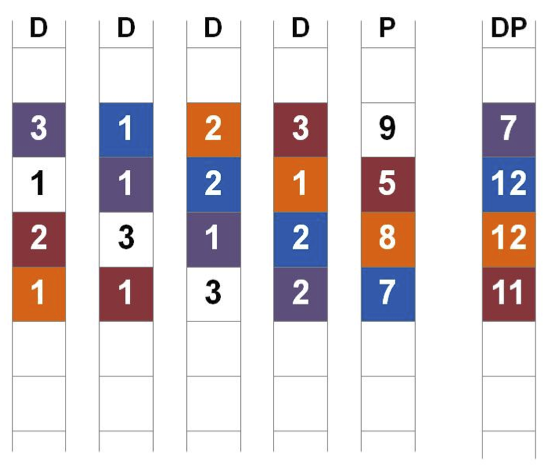
\includegraphics[ keepaspectratio = true]{media/raid-dp.png}
\mycaption{figure}{\label{abb:RAID-DP}NetApp RAID-DP doppelte Parität\cite{White2010}}
\end{center}


Als weiteren Schutzmassnahme vor Datenverluste, empfiehlt NetApp den Einsatz von Spare-Festplatten. Durch den Einsatz von Spare-Festplatten kann die Wiederherstellungszeit MTTR verkleinert werden, da die Wiederherstellung automatisch starten kann. Die Anzahl an Spare-Festplatten ist abhängig von der Anzahl Festplatten und Enclosure.

Die Datenverfügbarkeit kann mittels weiteren NetApp und der Snapmirror Funktion weiter erhöht werden. Dabei werden alle Änderungen an den Daten auf an eine weitere NetApp Synchronisiert. 

NetApp Speichert die Daten auf die Disk in 4 Kilo Byte Blocks. Zu jeden 4 Kilo Byte Block berechnet NetApp eine Prüfsumme und speichert diese in die Block Metadaten. Wenn der Block zu einen späteren Zeitpunkt wieder gelesen ist, berechnet die NetApp die Prüfsumme erneut und vergleicht diese mit der Gespeicherten Prüfsumme. Wenn die Prüfsumme nicht übereinstimmt, wird der Block mittels den Paritäts-Daten neu geschrieben, erneut gelesen und geprüft. Um die Integrität von Daten zu gewährleisten auf welche über eine langen Zeitraum nicht zugegriffen wird, wie diese zum Beispiel bei Archive Daten der Fall ist, hat NetApp eine konfigurierbare RAID durchkämmen (engl. RAID scrub) Funktion. Die Funktion geht durch alle Daten durch, wodurch die Prüfsumme von allen gespeicherten Daten geprüft wird. Die Funktion kann Zeitgesteuert oder wenn das System im Leerlauf befindet.\cite{Sundaram2006}

Zu beachten ist, dass die Prüfsumme auf dem Block nur auf der Speicherebene Wirkung hat. Fehler die in einer höheren Ebene stattfindet, wie zum Beispiel beim Einsatz von iSCSI zusammen mit einen Dateisystem, könnte bereits einen Fehler im Dateisystem durch einen Software Fehler oder Memory Fehler statt finden. 

NetApp bietet mehre Möglichkeiten eine Sicherungskopie der Daten herzustellen. Beim Einsatz von NFS oder iSCSI können die Daten über die Web-Servern mit einer Handels üblichen Sicherungs-Software gesichert werden. Bei NFS wird dazu die angefügten NFS Freigaben gesichert, bei iSCSI werden die Daten wie bei allen anderen Dateisystemen gesichert. Zubeachten ist jedoch, bei diesen verfahren, dass die Daten von der NetApp über den Server transferiert werden müssen, und dadurch der Web-Server mit dem Sicherungslast belastet wird. Neben der Sicherung der NetApp über den Server lässt sich die NetApp auch direkt sichern, dabei gibt es zwei Verfahren, mittels  Network Data Management Protocol (kurz NDMP) oder Mittels Snapshots. 

NDMP ist eines von NetApp mitentwickeltes Protokoll, welches für die Sicherung von NAS Geräte entwickelt wurde. Das Problem bei NAS Geräte ist, dass auf Ihnen ein dezidierte Betriebsystem läuft auf welche keine Installation eines Sicherungs-Agenten erlaubt, aus diesen Grund wurde das NDMP Protokoll entwickelt um eine allgemeines Agenten-Loses Sicherungsverfahren für NAS Geräte zu ermöglichen. NDMP wurde dem IETF im Jahr 2000 von der NDMP Initianden als Entwurf eingereicht, bis anhin ist jedoch noch kein RFC für NDMP Standardisiert. Trotzdem wird es von vielen NAS-Geräte- und Sicherungs-Software- Herstellern unterstützt. Eine Liste mit Sicherungs-Software Produkten, welche das NDMP Verfahren unterstützen gibt es auf der Webseite der NDMP Initianden\footnote{\url{http://www.ndmp.org/products/index.shtml#backup}} zu finden.\cite{NDMP.orga}\cite{NDMP.org}

Beim Snapshots Sicherungsverfahren werden zeitbezogene Sicherung des Dateisystem  erstellt. Bei den Snapshots wird nicht eine eigentliche Kopie der Daten bzw. Blöcke erstellt sondern die Referenz auf die Blöcke gespeichert. Wird nach dem erstellen eines Snapshots ein Block geändert wird die Änderung nicht im Original Block vorgenommen sondern in einen neuen Block und diesen Referenziert. Dadurch benötigt ein Snapshot minimalen Speicher, zudem lassen sich die Snapshots und damit die Sicherung in Sekunden erstellen unabhängig von der Anzahl Dateien oder der Verwendete Speicherkapazität. Durch den Einsatz von zwei NetApp Systemen und der SnapMirror Funktion kann, das ganze Dateisystem bzw. Volume inklusive aller Snapshots auf der zweiten NetApp gesichert werden. Die Sicherung mit Snapshots hat bei grossen Datenmengen entscheidende Vorteile, die Sicherung benötigt minimalen Speicherplatz, die Sicherung und Wiederherstellung ist innert Sekunden erstellt bzw. wiederhergestellt. Nachteile sind, dass der Speicherplatz mit der Sicherung bzw. Snapshots geteilt werden muss und das löschen der Daten zusätzlichen Speicherplatz verbraucht.

Sicherheit NFS IPSEC, intern

\subsection{Amazon S3}
Amazon zählt zu den Grössten, wenn nicht der grösste Online Speicheranbieter weltweit. Genaue Anzahlen über die Anzahl Kunden und Speicherkapazität veröffentlich Amazon nicht. Seit 2006 bietet Amazon Ihren Kunden unter den Produktname S3, einen Online Speicher an. Die genaueren Technischen Eigenschaften und Architektur des Online Speicher ist bis anhin von Amazon nicht veröffentlicht worden. Nach eigenen Angaben von Amazon basiert die Dienstleistung auf gewöhnlichen Computer Hardware.

Durch den Bezug des Speichersressourcen als Dienstleistung, fallen für den Kunden keine Investitionskosten in Hardware an. Zudem muss es sich nicht um die Wartung des Speichersystems kümmern. Dafür muss er allenfalls Kosten für die Anpassung der Applikation an das Amazon S3 API investieren, diese Kosten sollten jedoch in vergleich geringer ausfallen. Im Vergleich zum Betrieb eigener Speicherinfrastruktur wo der Kunde jeweils Speicherkapazitätsreserven haben muss, Zahlt der Kunde nur die effektive verwendete Speicherkapazität. Zudem fallen im keine Wartungskosten an um die Speicherinfrastruktur zu betreiben. Der Online Speicher von Amazon S3 gilt als ausgereiftes und etabliertes Produkt im Markt, weshalb davon ausgegangen werden kann, dass die Dienstleistung über die nächsten vier Jahre drübenraus noch bestehen wird und für den Kunden keine Migration notwendig ist. Amazon S3 wird ebenfalls von SmugMug ebenfalls eine Photodienstleister oder andere bekannte Web-Applikationen wie Dropbox verwendet.\cite{SmugMug}\cite{Dropbox2011}

Der Online Speicher Markt ist im Verhältnis zu anderen Speicher Märkte noch relativ jung, Analysten wie Jeff Boles gehen davon aus, dass der Online Speicher Markt in den nächsten Jahren weiter stark wächst. Wie in der Marktstudie beschrieben konnte Amazon seit dem Start des Amazon S3 Produktes die Anzahl gespeicherte Objekte jeweils pro Jahr mehr als verdoppeln (sie dazu \refabb{abb:AnzahlObjekteAmazonS3}). Die Konkurrenz von grossen Anbietern wie Google, Microsoft oder Rackspace nimmt für Amazon bereits zu. Für den Kunden bedeutet diese, dass die Anbieter Ihre Preise noch stärker kalkulieren müssen um ein Konkurrenz fähiges Angebot zu haben. Amazon hat die Preise für S3 Speicher erst kürzlich angepasst.\cite{Boles2011}\cite{Barr2012a}

Bei Online Speicher wie Amazon S3, kann der Kunde gleich nach Anmeldung an den Dienst, die Speicherressourcen verwenden. Es fallen also keine Installation von für
die Speicherinfrastruktur an. 

Die Daten können bei Amazon in mehren Regionen gespeichert werden. Zu den verfügbaren Regionen gehören, US Standard, US West (Oregon), US West (Northern California), EU (Ireland), Asia Pacific (Singapore), Asia Pacific (Tokyo), South America (Sao Paulo). Gemäss Amazon verlassen die Gespeicherten Daten eine Region nicht, ausser für die Erfüllung von Gesetzen oder auf Anforderung von Regierung Anweisung. Als US Amerikanisches Unternehmen steht Amazon wegen dem Patrot Act, unter der Pflicht, den USA Behörden Zugang zu Informationen zu gewährleisten auf behördlichen Anforderungen, auch wenn diese Informationen ausserhalb der USA gespeichert sind. Gemäss EU Recht darf jedoch keine gespeicherten Informationen, an dritten Zugänglich gemacht werden oder ausserhalb der EU gespeichert werden, ohne Einverständnis. Bei Microsoft ebenfalls eine Grosser Cloud Anbieter bestätigt diese Annahme, das die Daten nicht vor den Zugriff der USA geschützt sind.\cite{Amazon2012}\cite{Ostler}

Amazon S3 Speichert die Daten auf mehren Geräten in Verschiedenen Rechenzentren in der selben Region ab. Bei speichern werden die Daten Synchron in Verschiedene Rechenzentren gespeichert bevor die Speicherung als erfolgreich gemeldet ist, damit ist sicher gestellt, dass die Daten von beginn weg Redundant gespeichert sind. Die Integrität der Daten wird mit einer Prüfsumme sichergestellt. Die gespeicherten Daten werden von Amazon regelmässig auf Ihre Integrität geprüft und bei bedarf von einer Integer Kopie der Daten ersetzt. Mit diesen Massnahmen gewährleistet Amazon gemäss Dienstgütevereinbarung eine Zuverlässigkeit von 99.999999999\%. Bei bedarf kann die Zuverlässigkeit für Daten welche wenig Schutz benörigen, wie zum Beispiel Thumbnails von Bilder, mit einer geringeren Zuverlässigkeit von 99.99\% zu einen günstigeren Preis gespeichert werden.\cite{Amazon2007}

Durch die Redundante Speicherung der Daten auf mehre Geräten gewährleistet Amazone gemäss Dienstgütevereinbarung von 99.99\% pro Monat

Der Zugriff auf die Daten findet über eine API oder über die Verwaltungskonsole von Amazon statt. Für den Zugriff mit einen API bietet Amazon ein \gls{REST} und ein \gls{SOAP} Schnittstelle an. Der \gls{REST} Zugriff findet über HTTP statt, dabei werden Standard HTTP requests verwendet. Für den Zugriff kann auch einen gewöhnlichen Web-Browser verwendet werden solange die Objekte Öffentlich sind.

Einen Offiziellen POSIX IO Zugriff von Amazon steht nicht zur Verfügung, es existiert jedoch eine Quelloffenes Projekt Namens s3fs\footnote{\url{https://code.google.com/p/s3fs/}} welche es ermöglicht eine Amazon S3 Speicher unter Linux zu mounten. \cite{S3fs}

Amazon S3 unterstützt das Lesen und Schreiben von mehren Systemen. Beim Lesen einen Objekts welche von mehren Systemen Zugegriffen wird und beschrieben, stellt Amazon S3 die Lese konsistent sicher.\cite{Amazon2012a}

Im Amazon S3 können eine unbegrenzte Zahl von Objekten gespeichert werden, welche eine Speichergrösse von 1 Byte bis zu 5 Terrabyte haben können, wobei aber in einen PUT maximal 5 Gigabyte hochgeladen werden können. Für das Hochladen von Grösseren Objekten, muss die Multipart Funktion verwendet werden, welche das Objekte in mehren Teilen hochladet.\cite{Amazon2012b}

Die Daten können Verschlüsselt per SSL Zugegriffen bzw. gespeichert werden, somit ist gewährleistet, das dritte die Daten beim Transport nicht lesen können. Seit 2011 bietet Amazon kostenlos ebenfalls die Verschlüsselung mit AES-256 von Objekten im Speicher an. Dabei wird jedes Objekt mit einen eigenen Schluss ver- und entschlüsselt. Die erzeugten Schlüssel werden mit einen Master-Schlüssel ebenfalls Verschlüsselt und auf den Amazon-Servern gespeichert. Das Schlüsselmanagment bleibt jedoch bei Amazon, weshalb man abhängig von den Massnahmen zum schuzt des Schlusselmanagment die Amazon trifft. Wird diese Kompromittiert oder fällt aus ist der Zugriff auf die Verschlüsselten Daten nicht mehr möglich.\cite{RobertLippert2011}

Die Berechtigung auf gespeicherte Objekte oder Ordner können mit einen Rechte-Management verwaltet werden. Objekte können öffentlich zugänglich gemacht werden oder nur an bestimmte Authentifizierte Benutzer zur Verfügung gestellt werden. Zudem lassen Sich Zugriffe auf Objekte Protokollieren.\cite{Amazon2012b}

Für das Einlesen von Grossen Datenmengen bietet Amazon einen kostenpflichtigen Import/Export Dienstleistung an. Bei dieser Dienstleistung sendet der Kunde die Daten gespeichert auf  einen tragbares Speichergeräte an Amazon, welches die Daten direkt in Ihre Cloud ohne Umwege über das Internet einliesst.

Die API von Amazon ist gut Dokumentiert, weshalb für einen erfahrenen Entwickler die Anbindung der Web-Applikation an Amazon S3 umsetzbar sein sollte.

Für die Berechtigung und Verwaltung stellt Amazon ein Web-GUI zur Verfügung. Bis auf das eröffnen eines Speichers und die Initial Berechtigung sollten, wahrscheinlich nicht viel mehr Verwaltungsaufgaben anfallen.

Amazon bietet neben der Redundanz der Objekte kein weiteres Sicherungsverfahren an. Beim Herunterladen der Daten fallen für den Transfer weiter Kosten an.

\subsection{Gluster}

